\section{Data Visualisation}
To make sense of the vast amounts of data, to study trends, patterns and various other characteristics, Visualisation serves as an indispensable tool. Data Viz. in itself is another vast domain of study, yet it has its uses in Physics. Graphs are fundamental in Physics followed by images and animations. Here, I deal with \textbf{Graphs, Density Plots, Scatter Plots and Images}.
\subsection{Graphs}
2D Graphs require datasets of points to be represented on a coordinate plane. One often encounters such datasets in Physics, having data regarding a dependent variable changing with an independent one. However, to plot functions, we need to evaluate them at a linear space of points between the required range to produce illusion of continuity. The computer draws straight-lines between the points. So the end-result is not smooth but a set of line-segments. However, sampling the functions at hundreds of such points enables the creation of smooth-looking curves.\medskip \\
\par The underlying code plots functions of form $r=f(\theta)$, i.e. explicit in $r$ and $\theta$.
\\
\\ \\
\begin{lstlisting}[language=Python, caption=Polar Plot, frame=single ]
import numpy as np
import matplotlib.pyplot as plt
%matplotlib qt5 #for jupyter notebooks only


thetas=np.linspace(#range of theta, #number of sample points) 
def cart(theta, r):
	x=r*np.cos(theta)
	y=r*np.sin(theta)
	return (x,y)
def func(theta):
	return #function here

X=[]
Y=[]
for theta in thetas:
	x,y=cart(theta, func(theta))
	X.append(x)
	Y.append(y)
plt.plot(Y,X, 'b')
plt.xlabel('X')
plt.ylabel('Y')
plt.title(# Function Name)
\end{lstlisting}
\begin{figure}[H]
	\centering
	\subfloat[$f(\theta)=e^{\cos \theta}-2\cos4\theta+\sin^{5} \dfrac{\theta}{12} $]{{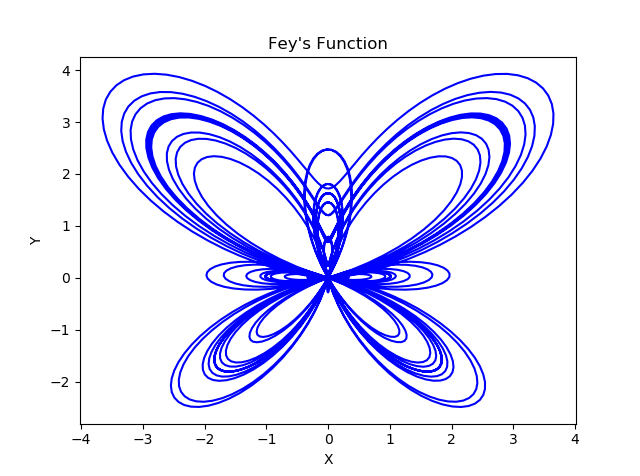
\includegraphics[width=7cm]{FeyFunc} }}%
	%\qquad
	\subfloat[$f(\theta)=\theta^{2}$]{{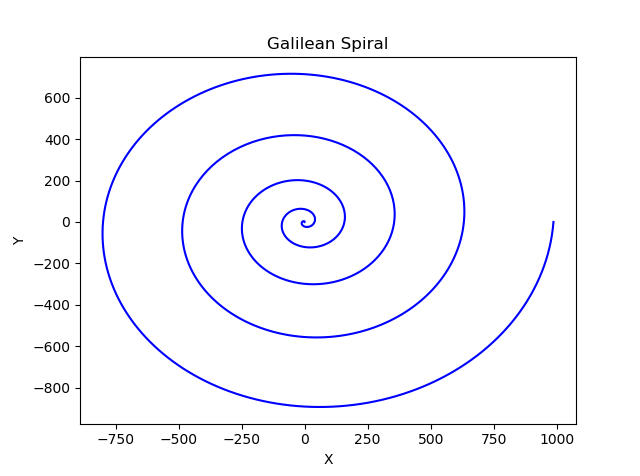
\includegraphics[width=7cm]{GalileanSpiral} }}%
	\caption{Polar Plots}%
	\label{fig:example}%
\end{figure}
\subsection{Density Plots and Images}
A \textbf{Density Plot} uses colours or brightness to represent magnitude on a 2D-Grid. In Python, we can pass an array of data, which can be 3D too. In this case, the values are interpreted as RGB values for each pixel in the grid. Consequently, many image formats are imported to Python in \textbf{3D-\textit{arrays}}. For instance, \textbf{FITS} (Flexible Image Transport System) is a widely used data format for storing astronomical observations by telescopes.\\
\par The underlying code displays the wave interference pattern for 2 plane waves produced in a medium at a particular separation.
\begin{lstlisting}[language=Python, caption=Interfernce Pattern, frame=single, label={lst:L2} ]
amp=1
wavelength=5
d=20
k=2*np.pi/wavelength
pond=np.zeros((500,500)) # two waves in a 1m*1m pond on a 500*500 grid
def dist(p1,p2):
	x1,y1=p1
	x2,y2=p2
	x1=conv_units(x1)
	x2=conv_units(x2)
	y1=conv_units(y1)
	y2=conv_units(y2)
	return ((x2-x1)**2+(y2-y1)**2)**(0.5)
def height1(p):
	return amp*np.sin(k*dist(p1,p))
def height2(p):
	return amp*np.sin(k*dist(p2,p))
def conv_units(point):
	return point/5
def conv_units2(point):
	return point*5
def height(p):
	return height1(p)+height2(p)
p1=(250,200)
p2=(250,200+conv_units2(20))
for i in range(500):
	for j in range(500):
		pond[i][j]=height((i,j))
pond=pond/2
plt.imshow(pond,interpolation='bicubic')
\end{lstlisting}
\begin{figure}[H]
	\centering
	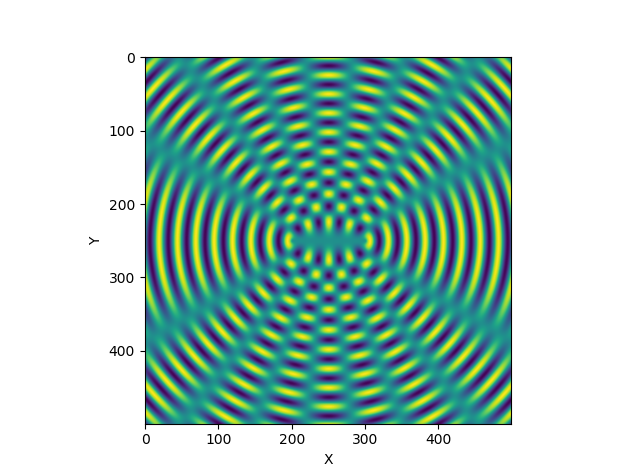
\includegraphics[width=0.7\linewidth]{WaveInterference}
	\caption{OUTPUT for Listing \ref{lst:L2}}
	\label{fig:waveinterference}
\end{figure}